\documentclass[12pt, a4paper]{article}

\usepackage[hmargin=2.5cm, vmargin=2cm]{geometry}
\usepackage{amsthm, amssymb, mathtools, yhmath, graphicx}
\usepackage{fontspec, type1cm, titlesec, titling, fancyhdr, tabularx}
\usepackage{color}
\usepackage{unicode-math}
\usepackage{float}
\usepackage{subfig}
\usepackage{hhline}
\usepackage{comment}
\usepackage[abbreviation,per-mode=symbol]{siunitx}
\usepackage{csvsimple}
\usepackage{subcaption}

\usepackage[CheckSingle, CJKmath]{xeCJK}
\usepackage{CJKulem}
\usepackage{enumitem}
\usepackage{tikz}
\usepackage[siunitx]{circuitikz}
\usepackage{wrapfig}
%\setCJKmainfont[BoldFont=cwTex Q Hei]{cwTex Q Ming}
%\setCJKsansfont[BoldFont=cwTex Q Hei]{cwTex Q Ming}
%\setCJKmonofont[BoldFont=cwTex Q Hei]{cwTex Q Ming}
\setCJKmainfont[BoldFont=cwTeX Q Hei]{cwTeX Q Ming}

\def\normalsize{\fontsize{12}{18}\selectfont}
\def\large{\fontsize{14}{21}\selectfont}
\def\Large{\fontsize{16}{24}\selectfont}
\def\LARGE{\fontsize{18}{27}\selectfont}
\def\huge{\fontsize{20}{30}\selectfont}

%\titleformat{\section}{\bf\Large}{\arabic{section}}{24pt}{}
%\titleformat{\subsection}{\large}{\arabic{subsection}.}{12pt}{}
%\titlespacing*{\subsection}{0pt}{0pt}{1.5ex}

\parindent=24pt

\DeclarePairedDelimiter{\abs}{\lvert}{\rvert}
\DeclarePairedDelimiter{\norm}{\lVert}{\rVert}
\DeclarePairedDelimiter{\inpd}{\langle}{\rangle}
\DeclarePairedDelimiter{\ceil}{\lceil}{\rceil}
\DeclarePairedDelimiter{\floor}{\lfloor}{\rfloor}

\newcommand{\unit}[1]{\:(\text{#1})}
\newcommand{\df}[1]{\mathop{}\!\mathrm{d^#1}}
\newcommand{\img}{\mathrm{i}}
\newcommand{\dD}{\mathrm{d}}
\newcommand{\dI}{\,\mathrm{d}}
\newcommand{\paral}{\mathbin{\|}}

\title{ \bf {\Huge 電子電路實驗5:Differential Amplifiers }\\ 實驗結報}
\author{B02901178 江誠敏}

\begin{document}

\maketitle


\section{實驗結果}

\subsection{Differential Gain}
\begin{figure}[H]
\begin{center}
  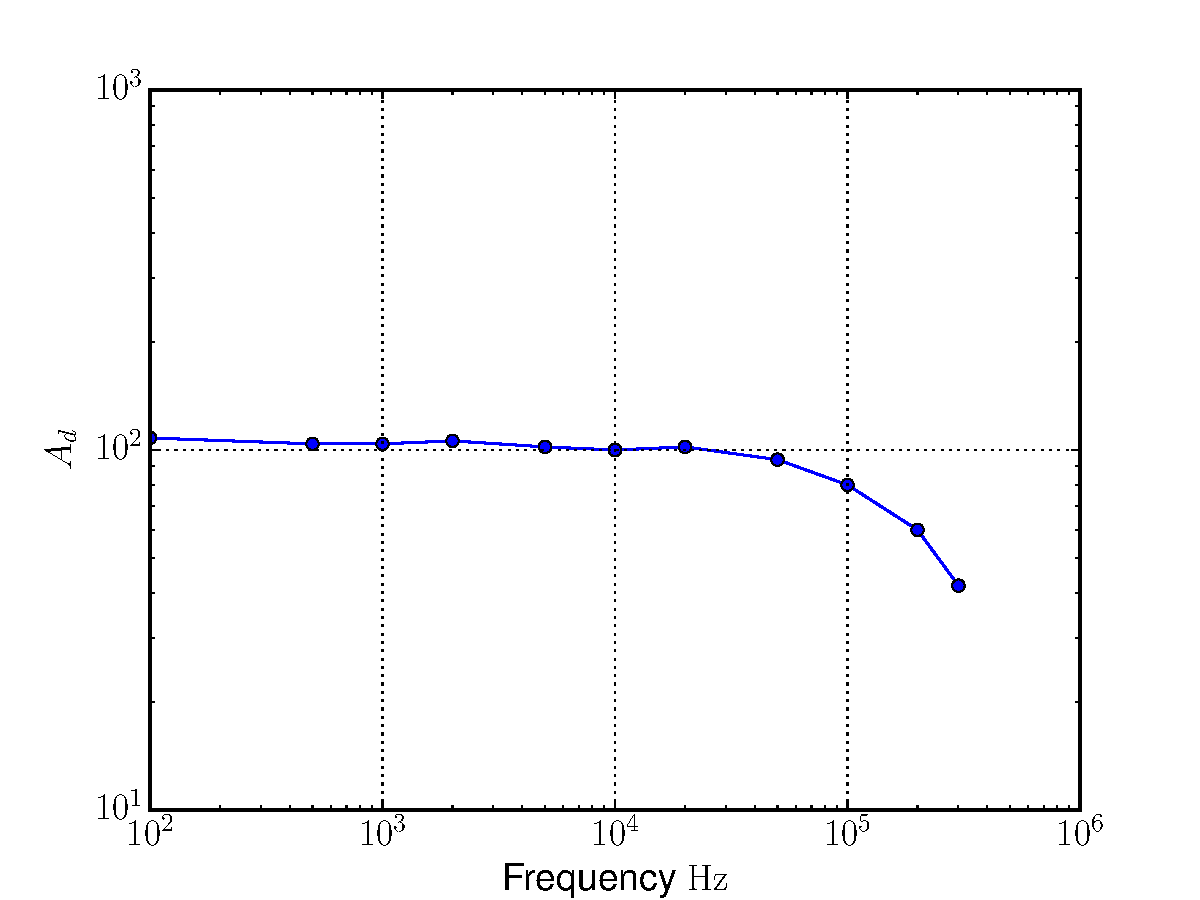
\includegraphics[width=.7\textwidth]{fig_ad.pdf}
\end{center}
\caption{$A_{d}$ Blot plot.}
\label{fig:}
\end{figure}
\subsection{Common Gain}
\begin{figure}[H]
\begin{center}
  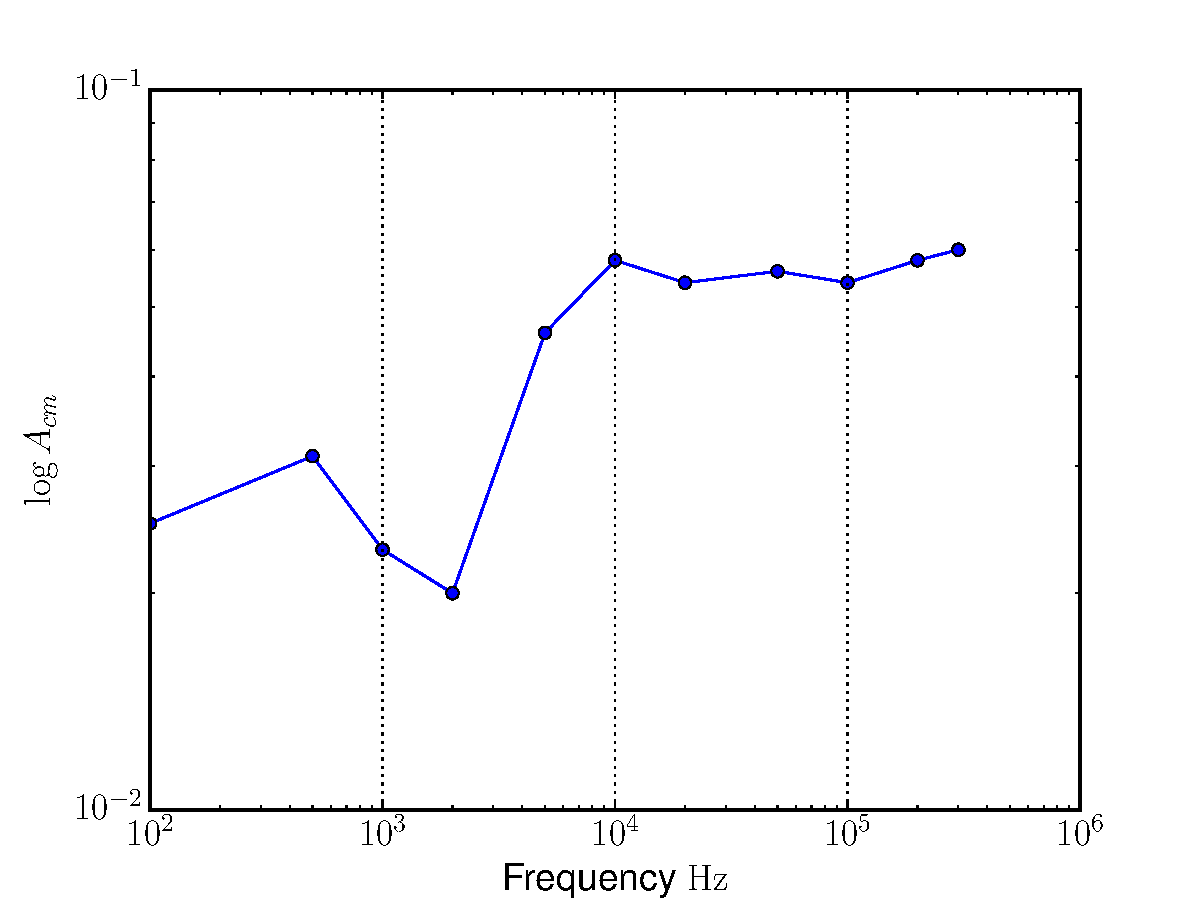
\includegraphics[width=.7\textwidth]{fig_acm.pdf}
\end{center}
\caption{$A_{cm}$ Blot plot.}
\label{fig:}
\end{figure}
\subsection{CMRR}
\begin{figure}[H]
\begin{center}
  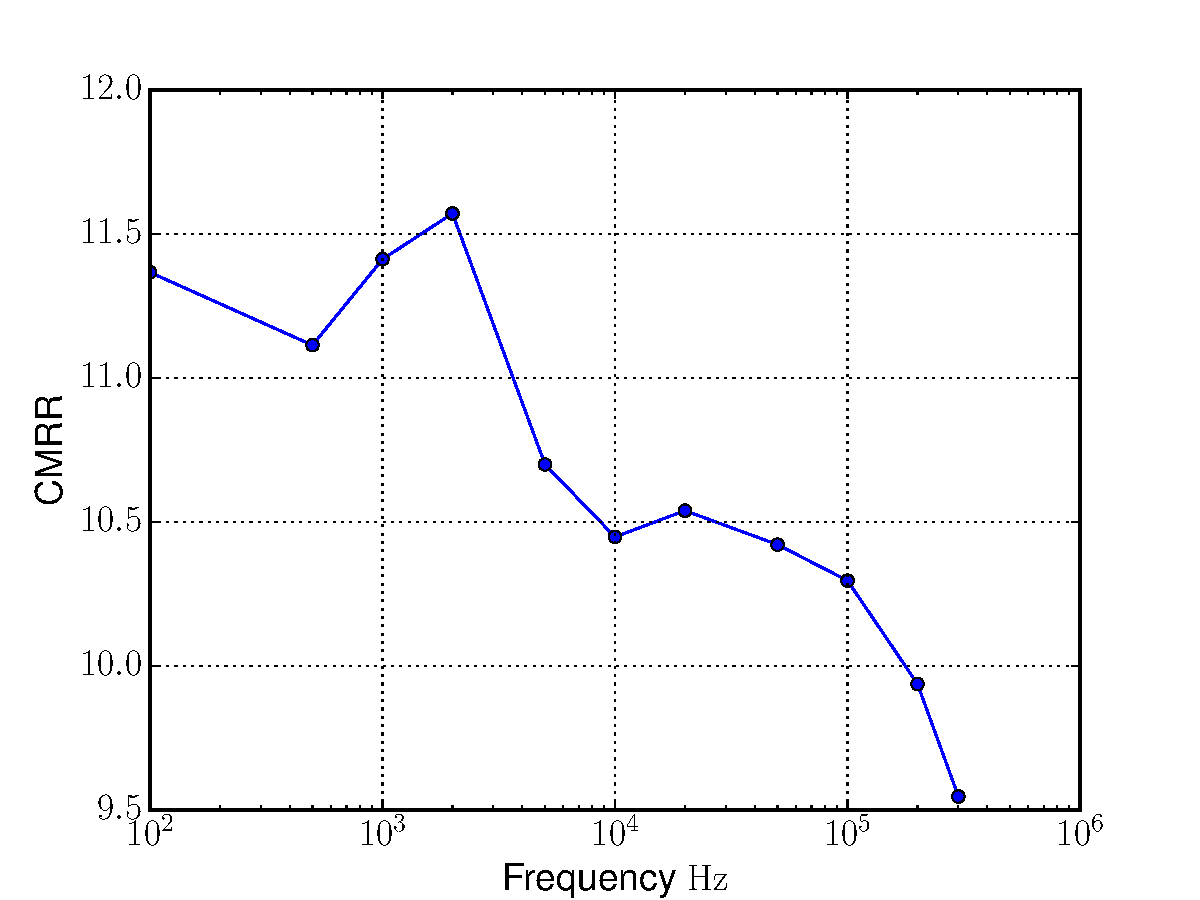
\includegraphics[width=.7\textwidth]{fig_cmrr.pdf}
\end{center}
\caption{CMRR}
\label{fig:}
\end{figure}


\clearpage
\section{結報問題}

\begin{enumerate}[itemsep=20pt, topsep=10pt]

  \item {In Fig. 4, the differential mode input and common mode input can be adjusted independently and not be interfered for each other.
    Let $I = \SI{1}\mA, R_{C1} = R_{C2} = \SI{10}\kohm$.Use PSIPCE to find: } \\[10pt]
    答:
    \begin{enumerate}[(a)]
      \item Transfer curve, where the input range of differential mode is around $\pm \SI{50}\mV$,
        and the internal resistor of the current source $R = \infty$. 
        \begin{figure}[H]
          \centering
          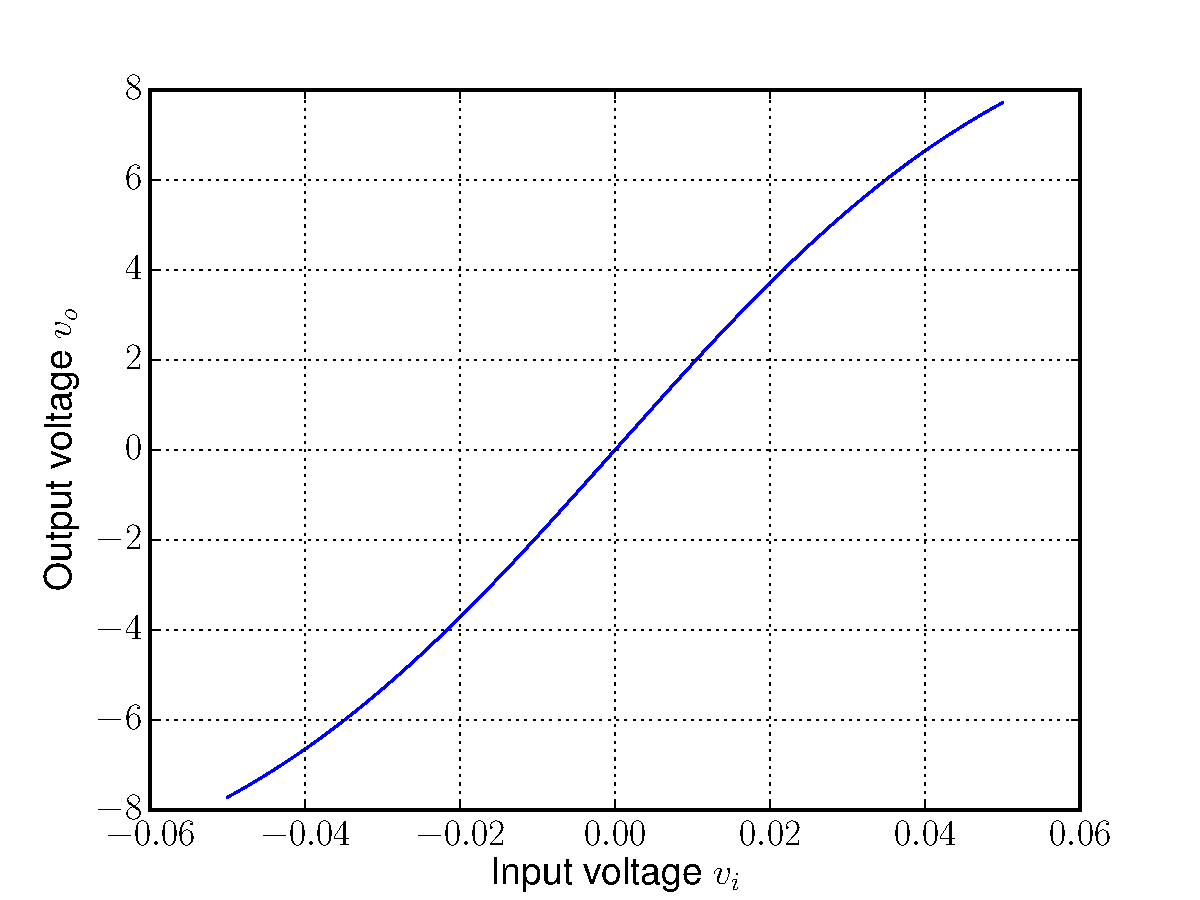
\includegraphics[width=0.65\textwidth]{ngspice/ad_vv.pdf}
          \caption{Transfer curve in differential mode}
          \label{fig:}
        \end{figure}

      \item $R_{id} \text{ and } A_d$, where the internal resist or of the current source $R=\infty$.
        \begin{figure}[H]
          \centering
          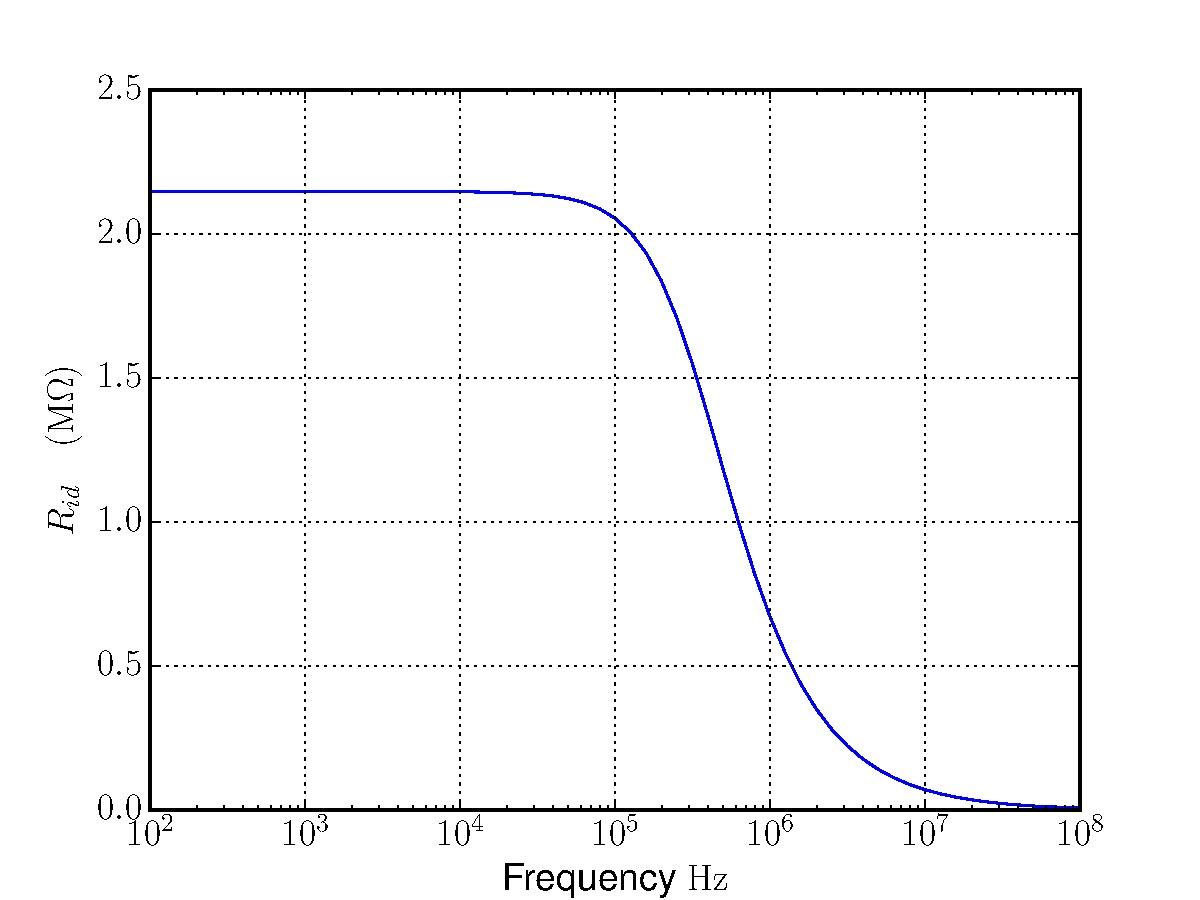
\includegraphics[width=0.65\textwidth]{ngspice/ad_r.pdf}
          \caption{Plot of $R_{id}$}
          \label{fig:}
        \end{figure}

        \begin{figure}[H]
          \centering
          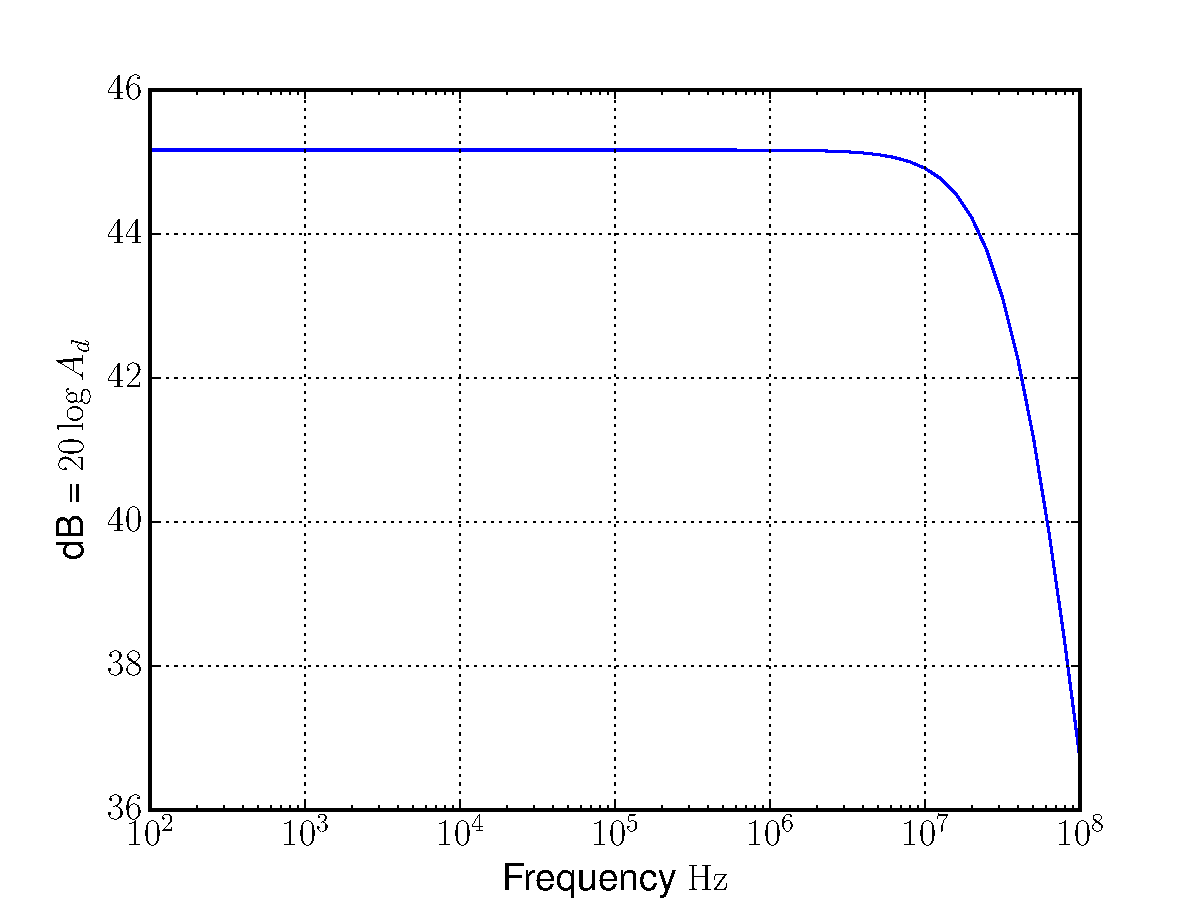
\includegraphics[width=0.65\textwidth]{ngspice/ad_db.pdf}
          \caption{Blod plot of $A_d$}
          \label{fig:}
        \end{figure}

      \item $R_{icm} \text{ and } A_{cm}$, where the internal resist or of the current source $R=\infty$.
        \begin{figure}[H]
          \centering
          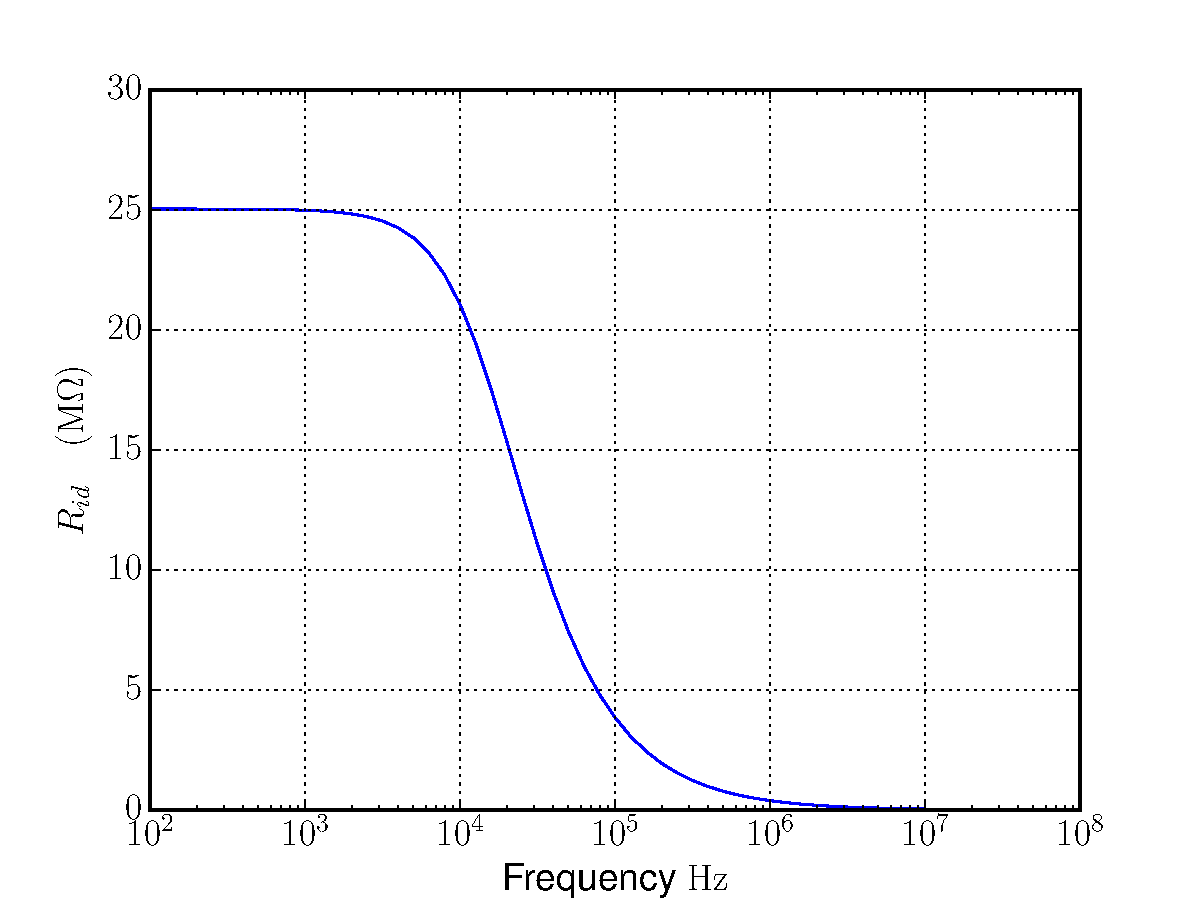
\includegraphics[width=0.65\textwidth]{ngspice/acm_r.pdf}
          \caption{Plot of $R_{icm}$}
          \label{fig:}
        \end{figure}
        Due to the symmetry of the circuit, $A_{cm}$ is $0$.
        \begin{figure}[H]
          \centering
          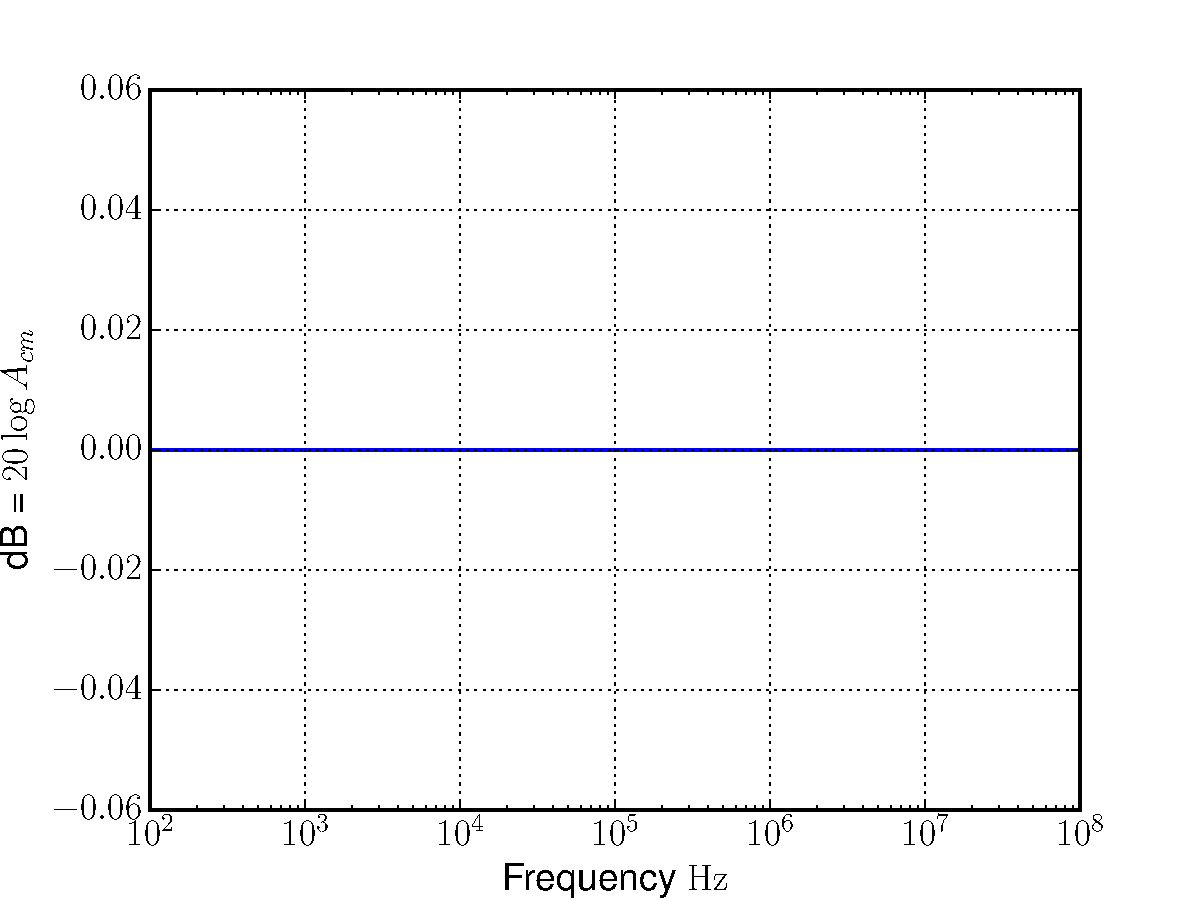
\includegraphics[width=0.3\textwidth]{ngspice/acm_db.pdf}
          \caption{Blod plot of $A_{cm}$}
          \label{fig:}
        \end{figure}

      \item $R_{icm} \text{ and } A_{cm}$, where the internal resist or of the current source $R=\SI{200}\kohm$.
        \begin{figure}[H]
          \centering
          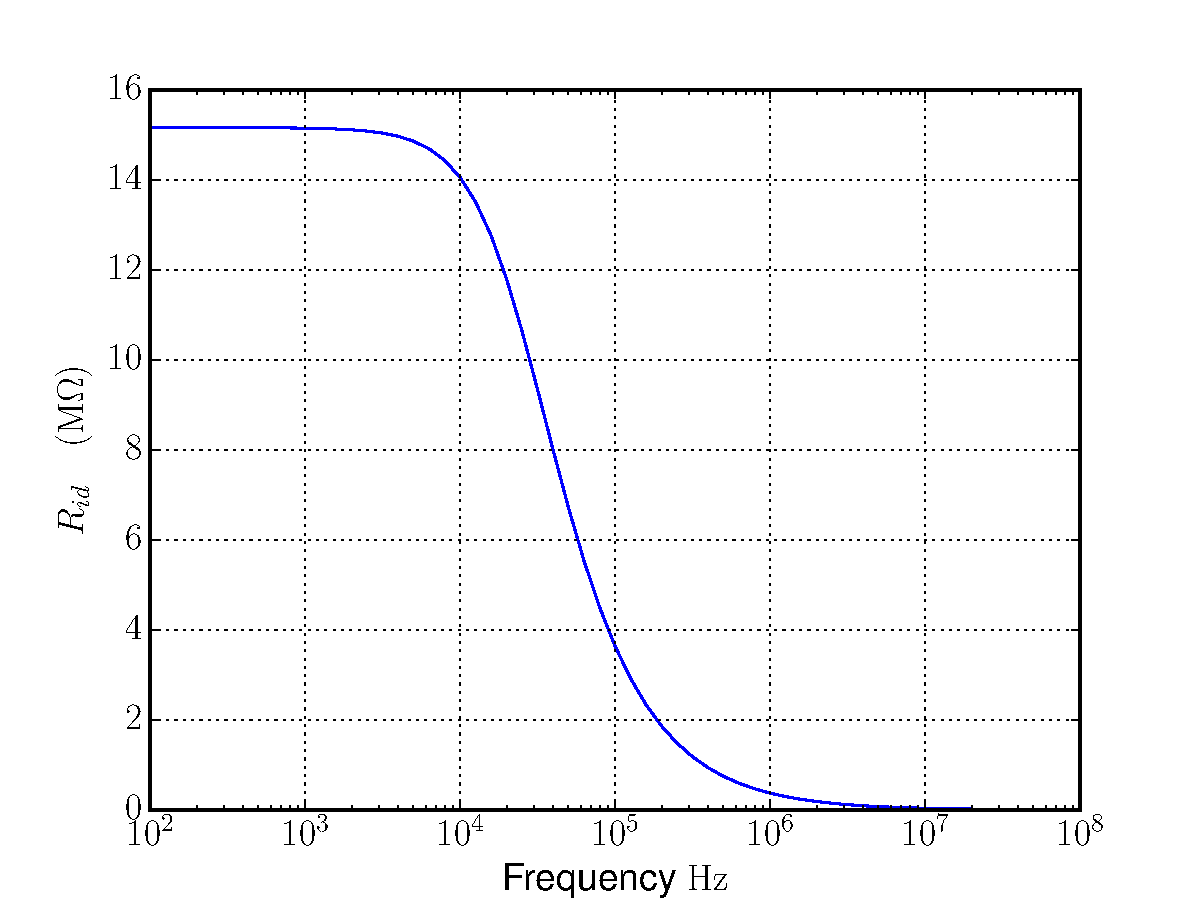
\includegraphics[width=0.65\textwidth]{ngspice/acmr200_r.pdf}
          \caption{Plot of $R_{icm}$}
          \label{fig:}
        \end{figure}
        Due to the symmetry of the circuit, $A_{cm}$ is $0$.
        \begin{figure}[H]
          \centering
          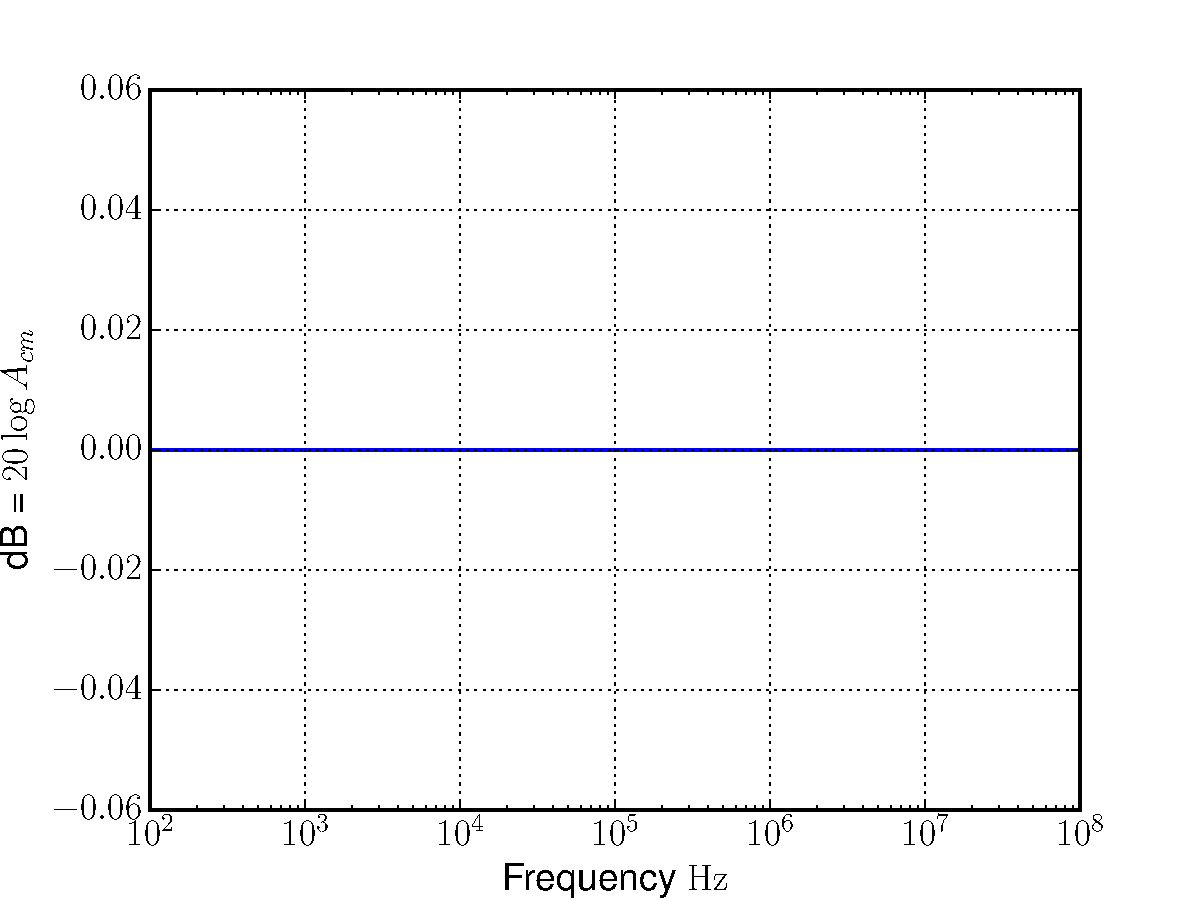
\includegraphics[width=0.3\textwidth]{ngspice/acmr200_db.pdf}
          \caption{Blod plot of $A_{cm}$}
          \label{fig:}
        \end{figure}
    \end{enumerate}
\end{enumerate}

\section{心得}
今天是自從上個月以來第一次開始做實驗。雖然過了很久記憶會模糊,不過我們都還記得
一件事情:出了問題,換儀器就對了!本來以為這樣就可以早早做完實驗早早去吃飯,沒
想到我在檢查的時候,波形變成麥當勞波形,當場被打回票。最後弄一弄才知道原來是示
波器的線鬆了。然後我們要去吃飯時店也幾乎都關了,只好去麥當勞怒吃雞塊了。
\end{document}

